\documentclass[../electromagnetism.tex]{subfiles}
\begin{document}
\section{Reflection and Refraction at a Spherical Surface}
\subsection{Mirrors}
Virtually, every surface of an optical instrument can be bunched up in two categories
\begin{itemize}
\item Plane surfaces
\item Curved surfaces
\end{itemize}
The path taken by light when interacting can be conveniently treated using ray theory, or geometric optics.\\
Consider two main cases now: 
\begin{enumerate}
\item Reflection by a spherical surface
\item Refraction through a spherical surface separating 2 different mediums
\end{enumerate}
Consider in both cases the origin of the ray as a point source $P$. Said $O$ the intercept of the line that connects the mirror to the source and called $Q$ the point where the beam intercepts the line $OP$ as in figure.
\begin{figure}[H]
	\centering
	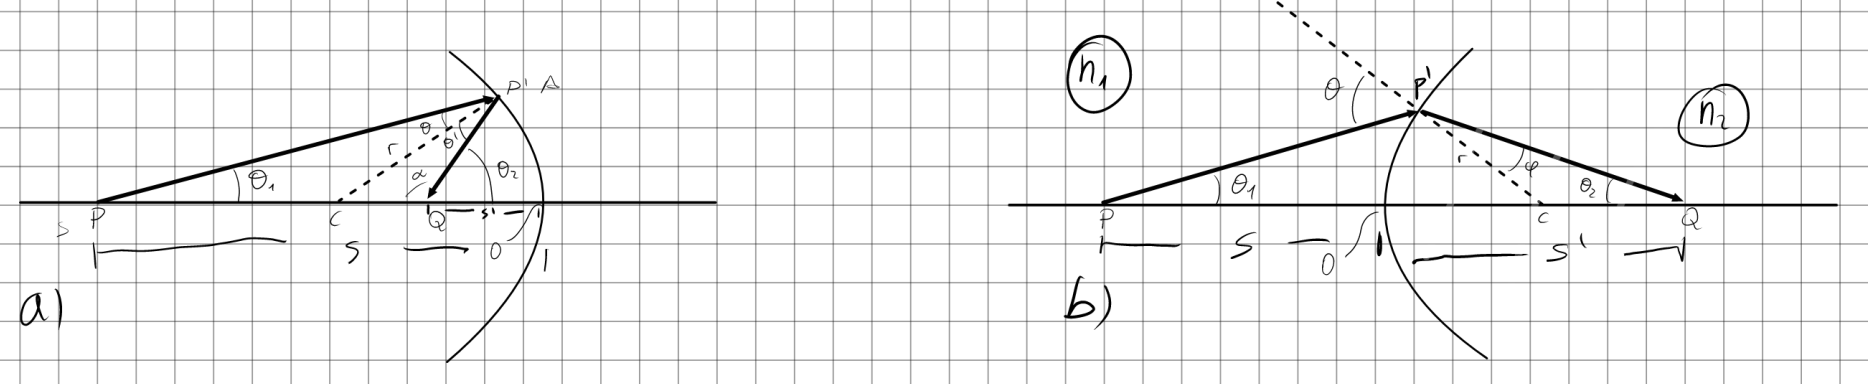
\includegraphics[width=\linewidth]{mirrors.png}
	\caption{The two configurations described above}
	\label{fig:curvedmirrors.gop}
\end{figure}
Call the distance $OP=s$ the \textit{object distance}, $OQ=s'$ the \textit{image distance} and the radius of curvature $OC=r$. We will have for the case of the spherical mirror that
\begin{equation*}
	PC=s-r\implies\frac{\sin\theta}{s-r}=\frac{\sin\theta_1}{r}
\end{equation*}
And
\begin{equation*}
	CQ=r-s'\implies\frac{\sin\theta'}{r-s'}=\frac{\sin\theta_2}{r}
\end{equation*}
Since we must have $\theta=\theta'$, we get the law of reflection for spherical mirrors
\begin{equation}
	\frac{r-s'}{s-r}=\frac{\sin\theta_1}{\sin\theta_2}
	\label{eq:refsph.gop}
\end{equation}
Analogously for the refracting surface we have 
\begin{equation*}
	r\sin\theta=(r+s)\sin\theta_1\qquad r\sin\phi=(s'-r)\sin\theta_2
\end{equation*}
Applying $n_1\sin\theta=n_2\sin\phi$ we get
\begin{equation}
	\frac{\sin\theta_1}{\sin\theta_2}=\frac{n_2}{n_1}\frac{s'-r}{r+s}
	\label{eq:trasph.gop}
\end{equation}
Where $n=\frac{n_2}{n_1}$.\\
Note how a bundle of rays originating from an axial point doesn't have the same focus. In fact the focus is function of $\theta_1$. This characteristic is typical of spherical optical surfaces and leads to what's known as \textit{spherical aberration}.\newpage
\subsubsection{General Mirror Equation and Focal Length}
Consider now the case of the source point placed at a height $h$ from the optical axis of the mirror. The image at the point $Q$ will then be at a height $h'$ from the same axis at the point $Q$ as in the next figure.\\
\begin{figure}[H]
	\centering
	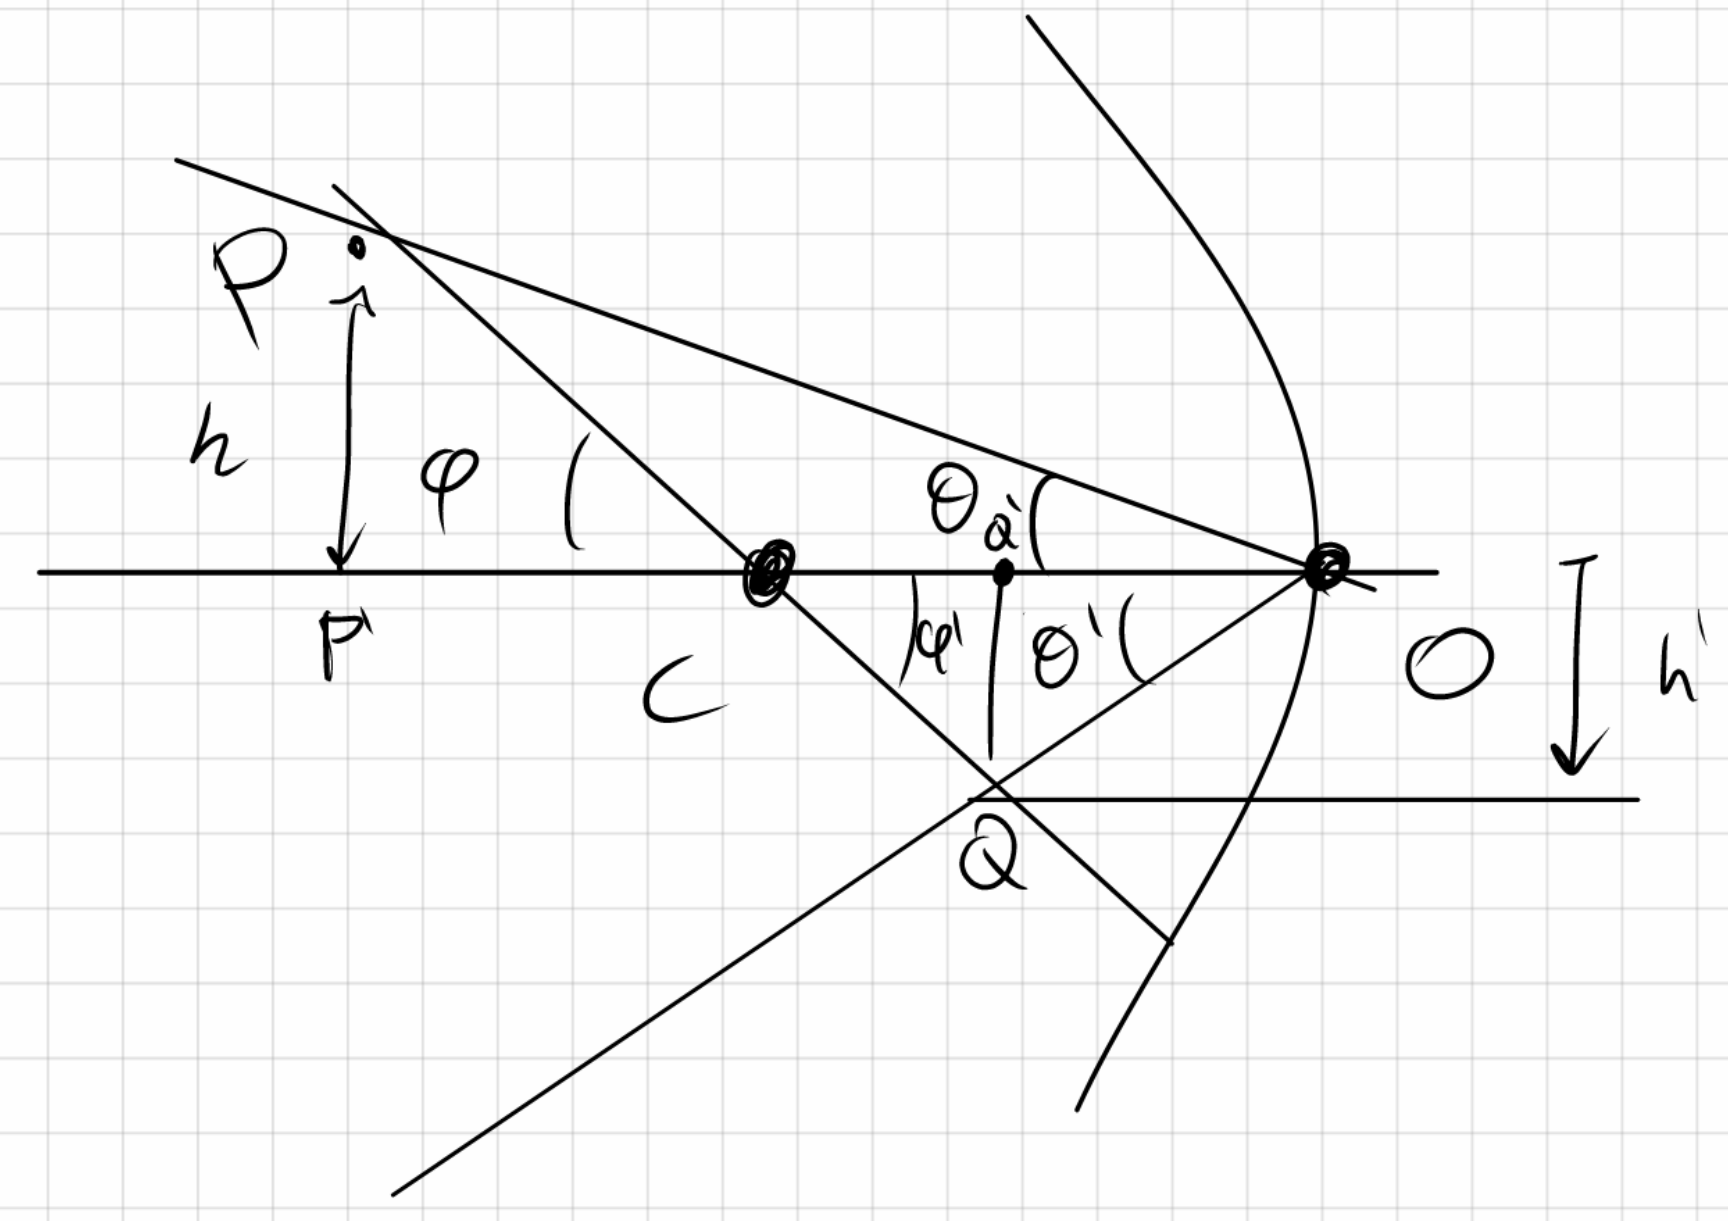
\includegraphics[width=\linewidth]{paraxial.png}
	\caption{Source offset by $h$, spherical mirror}
	\label{fig:paraxial.mir}
\end{figure}
From the previous figure, we can see two triangles which we can use for finding the relationship between the position of the source and the position of the image. Precisely we choose the triangles $PP'C$, $PP'O$ and the triangles $CQQ'$, $QQ'O$. Since $PP'=h$, $QQ'=h'$, $OP'=s$, $OQ'=s'$, $P'C=s-r$, $Q'C=r-s'$ we can say without doubts that
\begin{equation}
	\begin{paligned}
		\tan\theta&= \frac{h}{s}\\
		\tan\theta'&= \frac{h'}{s'}\\
		\tan\varphi&= \frac{h}{s-r}\\
		\tan\varphi'&= \frac{h'}{r-s'}
	\end{paligned}
	\label{eq:tangents.mir}
\end{equation}
Since it's also true that 
\begin{equation*}
	\begin{paligned}
		\tan(\theta)&= -\tan(\theta')\\
		\tan(\varphi)&= -\tan(\varphi')
	\end{paligned}
\end{equation*}
We get that
\begin{equation*}
	\begin{paligned}
		\frac{h}{s}&= -\frac{h'}{s'}\implies\frac{h}{h'}=-\frac{s}{s'}\\
		\frac{h}{s-r}&= -\frac{h'}{r-s'}\implies\frac{h}{h'}=-\frac{s-r}{r-s'}
	\end{paligned}
\end{equation*}
Using the previous equalities we get 
\begin{equation*}
	\frac{s}{s'}=\frac{s-r}{r-s'}\implies\frac{r-s'}{s'}=\frac{s-r}{r}=1-\frac{r}{s}
\end{equation*}
Fixing the relationship with algebra we get finally
\begin{equation}
	\frac{r}{s}+\frac{r}{s'}=2\implies\frac{1}{s}+\frac{1}{s'}=\frac{2}{r}
	\label{eq:mirroreq.mir}
\end{equation}
This equation is \textit{exact}, and is commonly known as the \textit{general mirror equation}.
The chosen signs are \textit{merely a convention}.\\
We define the \textit{focus} $f$ of a mirror the convergence point of rays coming from a source placed at infinity. Imposing $s=\infty$ we then have
\begin{equation}
	\frac{1}{s'}=\frac{2}{r}=\frac{1}{f}
	\label{eq:focus.gop}
\end{equation}
In general, in geometric optics, for calculating the path of the rays in the method of \textit{ray tracing of the first order}, the so called \textit{paraxial approximation} is employed. In this approximation, the source is far enough to consider the approximation $\theta\approx\sin\theta\approx\tan\theta$. In this approximation, the general mirror equation \eqref{eq:mirroreq.mir}, with the definition of focal distance becomes
\begin{equation}
	\frac{1}{s}+\frac{1}{s'}=\frac{1}{f}
	\label{eq:paraxialmirr.mir}
\end{equation}
For a spherical mirror, the focus is at the half radius point, as we have proven now in paraxial approximation.\\
With the previous formula, it's also possible to evaluate the magnification and orientation of the reflected image.\\
\begin{equation}
	M=\frac{h'}{h}
	\label{eq:magnification.gop}
\end{equation}
Notice the sign here: if $M>0$ both $h, h'$ share the same sign and therefore the image is not flipped.\\
Another convention is given to the mirror radii. If the mirror is convex, as we defined before $r<0$ and the reflected image is called \textit{real}, while it's called virtual in the remaining case.\\
It's possible to redefine the magnification starting from the previous parameters and using the general mirror equation, getting
\begin{equation*}
	M=-\frac{f-s'}{f}
\end{equation*}
Which, after inserting the general formula becomes
\begin{equation}
	M=-\frac{s'}{s}
	\label{eq:generalmag.gop}
\end{equation}
In the second case of transmission through a convex lens, the solution is completely analogous, giving us the following mirror equation
\begin{equation}
	\frac{n_1}{s}+\frac{n_2}{s'}=\frac{n_2-n_1}{r}
	\label{eq:convexlens.mir}
\end{equation}
A thing which is not really clear from the previous evaluations, is that in general $s'\in\R$, therefore there might be configurations where $s'<0$ or also that $f<0$. In general, the convention used is that $r>0$ when the mirror is concave with respect to the source, and vice versa. Note how having a negative image distance in this framework simply means that the rays diverge.
\section{Lenses}
\subsection{Thin Lenses}
Consider a simple lens with radii $r_1, r_2$ and negligible thickness $d$. If the lens is immersed in air ($n_1=1$) and made of glass ($n_g$), with the help of the previous equations that when the ray passes through the first and second curved surfaces we have that
\begin{equation}
	\begin{paligned}
		\frac{1}{s_1}+\frac{1}{s_1'}&= \frac{n_g-1}{r_1}\\
		\frac{1}{s_2}+\frac{1}{s_2'}&= \frac{1-n_g}{r_2}
	\end{paligned}
	\label{eq:mirroreqn-thin1.lens}
\end{equation}
For the full lens the straightforward result is then
\begin{equation}
	\frac{1}{s}+\frac{1}{s'}=(n_g-1)\left( \frac{1}{r_1}-\frac{1}{r_2} \right)=\frac{1}{f}
	\label{eq:lensmaker.lens}
\end{equation}
The last formula is valid only in paraxial approximation, and it's known commonly as the \textit{Lensmaker formula}.\\
With the derivation that we used it's clear that with multiple lenses in contact, the \textit{total} focal distance can be calculated via inverse addition. Therefore, called $f_e$ the effective focal lens of an optical system, we can say
\begin{equation}
	\frac{1}{f_e}=\sum_{i=1}^N\frac{1}{f_i}
	\label{eq:contact-lensmaker.lens}
\end{equation}
Note that if we introduce a separation $l$ between two lenses, the equation should be modified accordingly, as follows
\begin{equation}
	\frac{1}{f_e}=\frac{1}{f_1}+\frac{1}{f_2}+\frac{l}{f_1f_2}
	\label{eq:distance-lensmaker.lens}
\end{equation}
\subsection{Thick Lenses}
Consider now the case of lenses which have a non-negligible thickness $d$. Here, the object and image distance are measured from the position of two \textit{principal planes} placed at distances
\begin{equation}
	\begin{aligned}
		d_1&= fd\left( \frac{1-n}{r_2} \right)\\
		d_2&= fd\left( \frac{1-n}{r_1} \right)
	\end{aligned}
	\label{eq:principal-thick.lens}
\end{equation}
The focal length of the lens is evaluated from the following equation
\begin{equation}
	\frac{1}{f}=(n-1)\left[ \frac{1}{r_1}+\frac{1}{r_2}-d\frac{(n-1)^2}{nr_1r_2} \right]
	\label{eq:focal-thick.lens}
\end{equation}
\subsection{Chromatic and Spherical Aberration}
Due to the presence of dispersion all previous formulas are \textit{color dependent}. This kind of aberration is known as \textit{chromatic aberration} and can be corrected by using multiple lenses with different dispersion relations, such combination is known as an \textit{achromatic combination} and is obtained if and only if
\begin{equation}
	\begin{paligned}
		\delta_1=\frac{1}{n_1-1}\dv{n_1}{\lambda}&\qquad\frac{1}{n_2-1}\dv{n_2}{\lambda}\\
		f_1=f\left( 1-\frac{\delta_1}{\delta_2} \right)&\qquad f_2=f\left( 1-\frac{\delta_2}{\delta_1} \right)
	\end{paligned}
	\label{eq:achromatization.lens}
\end{equation}
Note that the process of achromatization of a lens is possible only in a finite interval of wavelengths.\\
One other typical aberration for lenses is the \textit{spherical aberration}. Here, we have that the focal distance also varies with the height of the rays with respect to the optical axis of the lens. Considering a paraxial ray hitting the lens at a height $h$ from the optical axis, the variation of focal length $\Delta f$ is
\begin{equation}
	\Delta f=\frac{1}{2}h^2f^2\frac{n-1}{n^2}\left[ \frac{1}{r_1^3}+\left( \frac{1}{f}+\frac{1}{r_2} \right)\left( \frac{n+1}{f}+\frac{1}{r_2} \right) \right]=\frac{1}{2}Kh^2
	\label{eq:difffocal-sph.lens}
\end{equation}
It's also possible to find that the minimum possible variation is 
\begin{equation}
	\Delta f_{min}\quad\text{ for }\quad\frac{r_1}{r_2}=\frac{n+4-2n^2}{n+2n^2}
	\label{eq:minab-sph.lens}
\end{equation}
\section{Ray Equations}
Considep a set of paraxial rays traveling in the general direction of the optical axis of an object, which we will indicate with $z$. The position and direction of any ray can be determined with only two parameters
\begin{enumerate}
\item The distance from the optical axis $\rho$
\item The angle between the ray and the optical axis $\theta$
\end{enumerate}
In the particular case of a free traveling ray, starting from a position $z_1$ to a position $z_1+d$, if at $z_1$ the ray is described by the parameters $(\rho_1,\theta_1)$, then, remembering that $\sin\theta\approx\tan\theta\approx\theta$
\begin{equation}
	\begin{pmatrix}
		\rho_2\\
		\theta_2
	\end{pmatrix}=\begin{pmatrix}
		\rho_1+\theta_1d\\
		\theta_1
	\end{pmatrix}
	\label{eq:freetravel.ray}
\end{equation}
If the ray passes through two different dielectrics, then at the boundary
\begin{equation}
	\begin{pmatrix}
		\rho_2\\
		\theta_2
	\end{pmatrix}=\begin{pmatrix}
		\rho_1\\
		\frac{n_1}{n_2}\theta_1
	\end{pmatrix}
	\label{eq:boundary-flat.ray}
\end{equation}
While, if the boundary is curved with curvature $R$
\begin{equation}
	\begin{pmatrix}
		\rho_2\\
		\theta_2
	\end{pmatrix}=\begin{pmatrix}
		\rho_1\\
		\frac{n_1}{n_2}\theta_1-\frac{\rho_1}{r}\left( 1-\frac{n_1}{n_2} \right)
	\end{pmatrix}
	\label{eq:boundary-curved.ray}
\end{equation}
Note that for lenses and curved mirrors, using the general mirror equation, it reduces to the simpler equation
\begin{equation}
	\begin{pmatrix}
		\rho_2\\
		\theta_2
	\end{pmatrix}=\begin{pmatrix}
		\rho_1\\
		\theta_1-\frac{\rho_1}{f}
	\end{pmatrix}
	\label{eq:mirror.ray}
\end{equation}
These vectors should not be confused with Jones vectors, but as for those, every interaction can be evaluated with $2\times2$ matrices known as \textit{ray matrices}. In general, we can define the following ray matrices for the previous interactions
\begin{equation}
	\begin{aligned}
		\begin{pmatrix}
			1&d\\0&1
		\end{pmatrix}&\qquad\text{free travel}\\
		\begin{pmatrix}
			1&0\\
			0&\frac{n_1}{n_2}
		\end{pmatrix}&\qquad\text{plane dielectric}\\
		\begin{pmatrix}
			1&0\\
			\frac{1}{R}\left( \frac{n_1}{n_2}-1 \right)&\frac{n_1}{n_2}
		\end{pmatrix}&\qquad\text{curved dielectric}\\
		\begin{pmatrix}
			1&0\\
			-\frac{1}{f}&1
		\end{pmatrix}&\qquad\text{thin lens / mirror}
	\end{aligned}
	\label{eq:useful-matrices.ray}
\end{equation}
Note that, as usual, if the system is composed by multiple smaller elements, like in the case of two lenses with focal lengths $f_1, f_2$, the total ray matrix of the system is
\begin{equation*}
	\begin{pmatrix}
		a&b\\c&d
	\end{pmatrix}=\begin{pmatrix}
		1&0\\-\frac{1}{f_1}&1
	\end{pmatrix}\begin{pmatrix}
		1&0\\-\frac{1}{f_2}&1
	\end{pmatrix}=\begin{pmatrix}
		1&0\\
		-\frac{1}{f_1}-\frac{1}{f_2}&1
	\end{pmatrix}=\begin{pmatrix}
		1&0\\
		-\frac{1}{f_e}&1
	\end{pmatrix}
\end{equation*}
Note how we gained again the result we found before
\subsection{Periodic Lenses and Resonators}
Ray matrices are fundamental in the study of multiple lens systems and resonators. We'll begin considering a system of two lenses with equal focal length $f$, uniformly distant $d$ between one another.\\
Considering the refraction of one lens and the subsequent free travel, we have that at the surface of the second lens the ray will be
\begin{equation}
	\begin{pmatrix}
		\rho_2\\\theta_2
	\end{pmatrix}=\begin{pmatrix}
		1&0\\-\frac{1}{f}&1
	\end{pmatrix}\begin{pmatrix}
		1&d\\0&1
	\end{pmatrix}\begin{pmatrix}
		\rho_1\\\theta_1
	\end{pmatrix}=\begin{pmatrix}
		1&d\\-\frac{1}{f}&1-\frac{d}{f}
	\end{pmatrix}\begin{pmatrix}
		\rho_1\\\theta_1
	\end{pmatrix}
	\label{eq:resfund.pr}
\end{equation}
Now consider a resonator, where the ray will pass multiple times through the system. One question we might ask is: \textit{is there a ray which is invariant for the system described?}\\
The answer is yes, and it can be determined via the usage of the spectral theorem. The secular equation for the last matrix is
\begin{equation}
	\det\begin{pmatrix}
		1-\lambda&d\\-\frac{1}{f}&1-\frac{d}{f}-\lambda
	\end{pmatrix}=\left( 1-\lambda \right)\left( 1-\frac{d}{f}-\lambda \right)=\lambda^2+\lambda\left( 2-\frac{\lambda}{f} \right)+1=0
	\label{eq:seceq.pr}
\end{equation}
Said $\alpha=1-\frac{d}{2f}$ we have that the equation simplifies notably, and gives the following result
\begin{equation}
	\lambda_{1,2}=\begin{dcases}
		-\alpha\pm\sqrt{\alpha^2-1}&\abs{\alpha}>1\\
		-\alpha\pm i\sqrt{1-\alpha^2}=e^{\pm i\phi}&\abs{\alpha}<1
	\end{dcases}
	\label{eq:eigenvalues.pr}
\end{equation}
Note that $\alpha\in\R$ by definition, and therefore $\lambda\in\Cf$. For a general eigenray of the system, after $N$ lenses, we have that
\begin{equation}
	\begin{pmatrix}
		\rho_N\\\theta_N
	\end{pmatrix}=\lambda^N\begin{pmatrix}
		\rho_1\\\theta_1
	\end{pmatrix}
	\label{eq:eigenray.pr}
\end{equation}
This system is the exact idea of system that we have in lasers. The idea of \textit{ray stability} is then clearly the need to have the beam as close as possible to the optical axis after $N$ passages. We thus prefer the case where $\abs{\alpha}\le1$, such that $\lambda^N=e^{\pm iN\phi}$. This result is then
\begin{equation}
	0\le1-\frac{d}{2f}\le1\implies\begin{dcases}
		0\le d\le4f&\text{lenses}\\
		0\le d\le2r&\text{mirrors}
	\end{dcases}
	\label{eq:stability.pr}
\end{equation}
Note that we \textit{always} need that $f\ge0$, therefore we are stuck to using converging or flat lenses or mirrors.\\
In the confocal configuration of the resonator, as for laser chambers, we need to have the focuses of the lenses/mirrors to coincide, i.e. $d=2f=R$, and the stability criterion is satisfied.\\
If the two lenses are different, then we will define two values of $\alpha$, as
\begin{equation*}
	\alpha_1=1-\frac{s}{2f_1}\qquad\alpha_2=1-\frac{d}{2f_2}
\end{equation*}
And the stability condition becomes
\begin{equation}
	0<\alpha_1\alpha_2<1
	\label{eq:differentstab.pr}
\end{equation}
\end{document}
%%TODO 23/01/23 2h43m0s
%%TODO 24/01/23 1h26m50s
%%TODO 25/01/23 0h0m0s
%%TODO 26/01/23 2h12m15s
%%TODO 27/01/23 55m48s<+time+>
